\chapter{The UK Light Injection System}
\label{chp:ukli}

As mentioned in Chapter 4, the Korean laser system is used to measure the scattering and absorbtion coefficients in Super-Kamiokande. The UK calibration group's efforts have been focussed on improving the data analysis method and improving the accuracy of the water coefficient measurements. To aid this effort a new UK developed Light Injection (UKLI) system was installed into Super-Kamiokande during the refurbishment that ocurred in the summer of 2018. The ultimate goal is to install the light injection system in Hyper-Kamiokande, which was the purpose of its initial development. The UK system has its own set of optics, which unlike the Korean system, involves optics with multiple beam spot diameters, which will be described in detail in this Chapter, along with the electronics involved in the production of the system. Much like the Korean laser system method of measuring the absorption and scattering measurements described in Chapter 4, the measurements from the UK system involves the generation of Monte Carlo specific to the diameter of the beam spots produced from the UKLI, the production methods of which will also be discussed in detail in this chapter. Much like for the Korean system, a monitoring system was introduced to observe the light injection output for the different optics, and was also of interest during the Gadolinium loading period to examine changes due to the addition of gadolinium sulphate in the detector. 

\section{The UK Light Injection System Electronics}

The electronics setup architecture for the UK Light Injection system is made of sixteen light emitting diode boards which are each coupled to three optical fibres, as well as a monitor PMT, an optical power meter and two motherboards as shown in Figure \ref{fig:ukli_system_architecture}. 

\begin{figure}
    \centering
    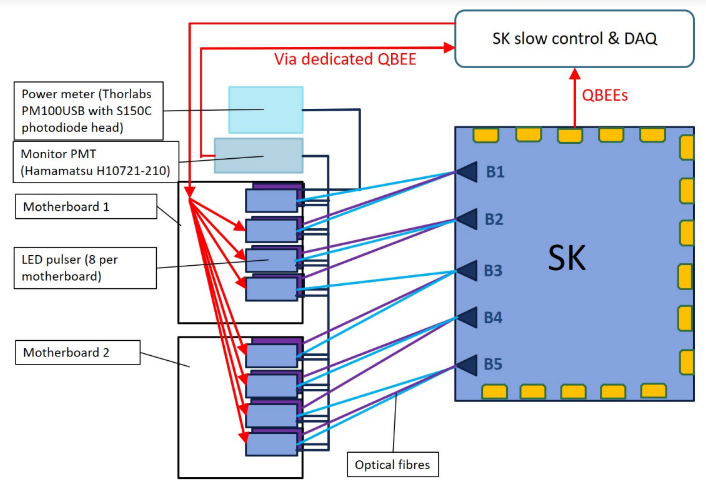
\includegraphics[width=0.7\textwidth]{Figures/ukli_system_architecture.png}
    \caption{UKLI electronics system architecture, showing optical fibre and motherboard couplings and QBEE connections.}
    \label{fig:ukli_system_architecture}
\end{figure}

The light being pulsed has a wavelength of 435 nm and is produced by light emitting diodes which are controlled by Field Programmable Gate Arrays and uses sixteen LED pulser boards placed on two motherboards (8 LED pulser boards on each) which controls which channel to send a signal to. Fifteen of the sixteen channels deliver light into the detector, while the remaining channel sends light to a seperate monitoring system. There are three optical fibres each LED is coupled to: firstly, a channel connected to the monitor PMT, secondly to an optical fibre which sends light into the Super-Kamiokande detector, and finally to the on-board photodiode monitor. The monitor PMT is a very small 2 inch Hamamatsu PMT which has a peak sensitivity to 400 nm wavelength light. A signal is sent from the light emitting diode to the monitor PMT and this information is sent to one of the QBEE (QTC-based electronics with Ethernet) channels for the detector - the charge recorded by the monitor PMT is meant to be used as a normalisation factor for calculations of the absorption and scattering water parameters. 
\newline

The monitor PMT is contained inside a custom made 3D printed box to make sure there is no external light reaching it. There are nineteen channels which monitor the input of the PMT, and these are kept in place against the PMTs photocathode. Fifteen of these fibres are connected to light emitting diodes which give light to the detector, one channel is coupled to the LED board for monitoring the system and the last three channels are reserve. The channel which is coupled to the LED board for monitoring of the syste is used for calibrating the monitor PMT, where the signal from this channel is inputted into the optical power meter. This fibre and the fifteen fibres that are connected to the LEDs that give light to the detector are linked to a photodiode monitor board (PMD). There are two PMDs per motherboard, therefore four in total, which record the output from the LED channels and can switch off a channel if it is producing light when it is not meant to which stops light leaking into the tank. 

\subsection{UKLI System Optics}

